\section{Methods Used}
We divided the first subtask in three subgoals: Finding the object; tracking the object and picking up the object. 

\subsection{Finding The Object}
To find the object we used a simple routine, in combination with a more complicated recognition. The routine is: Start flying at a low height, and then turn 360 degrees.
 While turning we constantly check the front camera (since we can only check one camera properly at the same time) for our object. If we had no indication of the object
at this particular height we would increase the search height and begin again.
If the object had been found we would store that height and go back to that when
the object was lost. This, in order to speed up the search process later on (it was not unknown for the \Ardrone to lose the object some times). \\

We chose to make an object that had a bright pink color. This simplified things
for us: We only had to recognize a big enough surface of our color. We tried a
	couple of things to recognize our color:\\

The first step was to define the values that our color ranged from. We chose to
divide our image in HSV values. This divides the image in 3 different layers:
Hue, Saturation and Value. These layers represent the values of the image's
``Hue, Saturation and Value'' as shown in figure \ref{HSV}. OpenCV changes these
values to a range of 0 to 255 (to create images it can show) by dividing the Hue
by 2, and the saturation and value by $\frac{100}{255}$. The advantage of HSV
above RGB (Red Green Blue) values is that it is easier to recognize if your
color needs to be a bit lighter (thus, increasing the Value) than that your
color needs to be a bit greener.\\

\begin{figure}
  \centering
      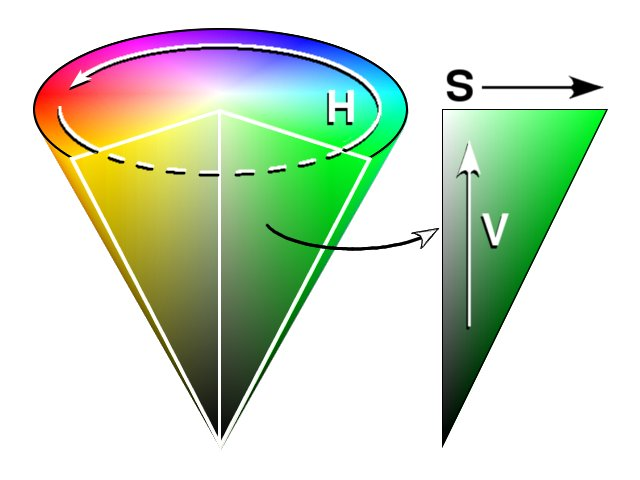
\includegraphics[scale=0.35]{HSV.jpg}
  \caption{Hue (H), ranging from 0 to 360 degrees; Saturation (S), ranging from 0 to 100\% and Value (V) ranging from 0 to 100\% }
  \label{HSV}
\end{figure}

OpenCV placed the pixels that were in the right HSV range in a new picture. This
picture had a value of 1 on the pixel where our color-values were good, and a
value of 0 where they were bad. This resulted in a white blob where almost every
white pixel was on our object. Something like figure \ref{processed}.
Unfortunately the computer can not understand this. We still need to let the
\Ardrone know where the object is in this picture. To find the centre of the
object, we tried histogram backprojection.

% persoonlijk vind ik dit mooier maar hij moet wel een wit randje ertussen bouwen 
% Je hebt gelijk. Ik had die andere manier als eerst gevonden op google, maar
% zocht eigenlijk deze. De whitespace zit er nou tussen.
\begin{figure}
  \centering
  \subfloat[The image after the first processing.]{\label{fig:processed}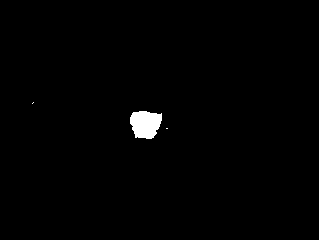
\includegraphics[width=2.1in]{processedImage}}
  \hspace{1cm}
  \subfloat[The image after the second processing.]{\label{fig:processed2}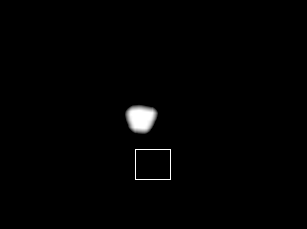
\includegraphics[width=2.1in]{processedImage2}}
  \caption{Results of processing a frame, the square in the right image debug-output.}
  \label{processed}
\end{figure}

\subsection{Tracking The Object}
Histogram backprojection is a technique that takes a histogram (a representation of the distribution of the colors in an image) of your target, and matches it for the
histogram of the same size of a part of the image around each position (x, y) in the image. Where the histogram of the target matches the histogram of some location in the
image a great deal, the location will have a big number. And, of course, it is the other way around for those locations that do not match. 
Unfortunately we experienced our first real problem with OpenCV, the function had a bug that we could never solve.  \\

Therefore we tried a different, somewhat simpler method, called ``Template Matching''. This is a bit like histogram backprojection, but instead of using histograms, we 
use a template of the object we wanted to see. This is is a somewhat less complicated method and it works a little bit less well but it did the trick. And 
since we allready had an image that was only black or white (0 or 1), our template simply had to be a white square. This would match the white space in our image, but not a
 single white pixel. This resulted in an image like in figure \ref{processed}. As you can see, the edges are a bit fuzzy. Now we can use the OpenCV function ``minMaxLoc'' 
to locate the centre of the object, which is the brightest pixel in the image.  \\
% we zouden hier nog de mooie formule van de opencv api in kunnen stoppen: 
% http://opencv.willowgarage.com/documentation/python/object_detection.html?highlight=template%20match

At first the size of our template was fixed. It was a 10 by 10 pixels square. This resulted in our second image having too many pixels with a value of 1 (and thus being 
the brightest). When we were able to calculate the distance of the object (see section \ref{sec:pickingUp}), we made the template size variable, meaning that we always 
exactly found the centre of the object. The result can be seen in figure \ref{fig:betterR}. 

\begin{figure}
  \centering
      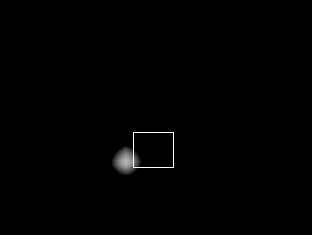
\includegraphics[scale=0.51]{betterR.png}
  \caption{The result of scaling the template image to the distance.}
  \label{fig:betterR}
\end{figure}


\subsection{Picking Up The Object}
We chose an object with a handle, and a hook on our \Ardrone. The advantage of this is that we do not have to hover above, or land on our object, but we can simply fly over it, and pick it up with the hook. This is a lot easier, because the \Ardrone has a flying error, which complicates hovering above the object. 

To be able to pick up the object we went through this routine:
\begin{itemize}
\item Put the centre of the object in a specified square (the white square in figure \ref{processed}). 
\item keep it there for a second, to compensate the flying error.
\item fly towards the target, while keeping it in the square
\item When the \Ardrone is close enough, switch to watching the bottom camera, fly a bit higher and fly forward, to pick up the object.
\end{itemize}
To be able to do these things, we had to do some tricky things:

\subsubsection{Calculate Distance}
The most important thing we did was calculating the distance to the object. The ammount of pixels that belong to our 
object should have some relation to the distance to the object because the object is smaller if we are further away
from it. So all We had to do was to count the number of non-zero pixels in the second processed
window. 
We calibrated this by counting the amount of those pixels for a number of known distances and
then used an online formula finder \footnote{\href{http://zunzun.com/FunctionFinder/2/}{Zunzun.com function finder}} to find the formula 
that calculates the distance. %See equation \ref{eq:distanceFormula}.

\begin{comment}
     # coefficients
       a = 7.6315999175901217E-01
       b = -6.4523069253280248E-04
       c = 8.3189620080930808E+01
       d = -1.5517143254934185E-01
       f = 1.4487053946697799E+00
       g = -4.6478934298555246E-03
       Offset = 2.1482272389707244E-01

       temp = a * math.exp(b*x_in) + c * math.exp(d*x_in) + f * math.exp(g*x_in)
       temp = temp + Offset
       return temp

\begin{equation}
willen we deze formule er ECHT in hebben?
\label{eq:distanceFormula}
\end{equation}
\end{comment}

\subsubsection{Variable Steering Commands}
Another important factor in moving towards the object were variable steering commands. 
It is really important to steer towards the object quickly once you can. The faster the 
better because the flying errors are quite enormous. It is not unusual to see the \Ardrone
drifting off quite a bit even if we only want to rotate it 360 degrees. However, once
the \Ardrone has positioned itself in front of the object it will overshoot with the
corrections if it drifts of. To compensate for this effect we made sure the strength
of the steering values are lower as the \Ardrone is closer towards the target. This
is the case for pitch, roll and even the gaz commands. For the yaw, we did
almost the same, but in stead of letting it depend on the object distance, we
let that depend on the place of the object in the picture. 

\subsubsection{Blind Flight}
The \Ardrone can only send one of the two video-streams over the network to our application. 
When we decide it is time to fly over the object, to pick it up, we switch to the bottom 
camera. This allows us to steer the \Ardrone in the right direction when we notice it drifting
off but in the mean time we do not see any of the more interesting data (the front view). If
we miss the object completely we might fly against a wall. To solve this we granted the
\Ardrone a limited amount of time on the bottom camera to pick up the object before we switch
back to the front camera and restore whatever it might have done. 

\label{sec:pickingUp}

























